\subsection{Unsicherheiten}\label{subsec:unc}

Jegliche Unsicherheiten werden nach GUM bestimmt und berechnet.
Die Gleichungen dazu finden sich in \ref{fig:GUM_combine} und \ref{fig:GUM_formula}.
Für die Unsicherheitsrechnungen wurde die Python Bibliothek "uncertainties" herangezogen, welche den Richtlinien des GUM folgt.
Alle konkreten Unsicherheitsformeln stehen weiter unten.
Für Unsicherheiten in graphischen Fits wurden die $y$-Unsicherheiten beachtet und die Methode der kleinsten Quadrate angewandt.
Dafür steht in der Bibliothek die Methode "scipy.optimize.curve\_fit()" zur Verfügung.

Für digitale Messungen wird eine Unsicherheit von $u(X) = \frac{\Delta X}{2\sqrt{3}}$ angenommen, bei analogen eine von $u(X) = \frac{\Delta X}{2\sqrt{6}}$.

\begin{description}
	\item[item] % TODO0
	
\end{description}
\begin{figure}[ht]
	\begin{equation*}	
		x = \sum_{i=1}^{N} x_i
		;\quad
		u(x) = \sqrt{\sum_{i = 1}^{N} u(x_i)^2}
	\end{equation*}
	\caption{Formel für kombinierte Unsicherheiten des selben Typs nach GUM.}
	\label{fig:GUM_combine}
\end{figure}

\begin{figure}[ht]
	\begin{align*}
		f = f(x_1, \dots , x_N)
		;\quad
		u(f) = \sqrt{\sum_{i = 1}^{N}\left(\pdv{f}{x_i} u(x_i)\right) ^2}
	\end{align*}
	\caption{Formel für sich fortpflanzende Unsicherheiten nach GUM.}
	\label{fig:GUM_formula}
\end{figure}

\subsection{Zusatz}\label{subsec:Zusatz}

\begin{figure}[ht]
	\centering
	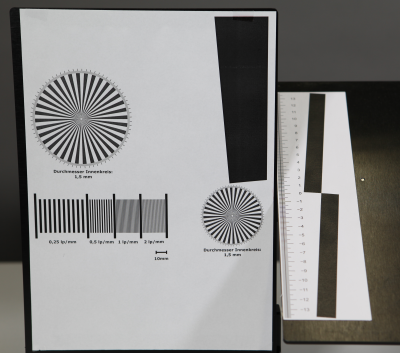
\includegraphics[width=0.7\textwidth]{bilder/testbild.png}
	\caption{sample.\cite{WWU}}
	\label{fig:testbild}	
\end{figure}	